\documentclass{beamer}

\title[Crisis] % (optional, only for long titles)
{}
\author[]{\small Markus Palacios \\ \emph{markus.palacios.5733@student.uu.se} \\ \and Jonathan Sharyari \\ \emph{jonathan.sharyari.0152@student.uu.se} \\  Peng Sun\\\emph{peng.sun.8197@student.uu.se}}
\usetheme[numbers]{Uppsala}
\subject{Computer Science}
\subtitle{Project Presentation}

\date[2015-03-13] % appears in the bottom of the sidebar
{March $13^{th}$, 2015}
\institute[Dept. of Information Technology] % appears in the footline
{
	Department of Information Technology\\
		Uppsala University
}

\usepackage{biblatex}
%\setbeamertemplate{footline}[text line]{%
	%  \parbox{\linewidth}{\vspace*{-8pt}Algorithmic Verification of Channel Machines\hfill- \insertpagenumber -\hfill\insertshortauthor}}
	%\setbeamertemplate{navigation symbols}{}

\begin{document}
\begin{frame}[plain]
\titlepage
\end{frame}

\section{Assignment 1}
\begin{frame}
	\begin{figure}[h!]
	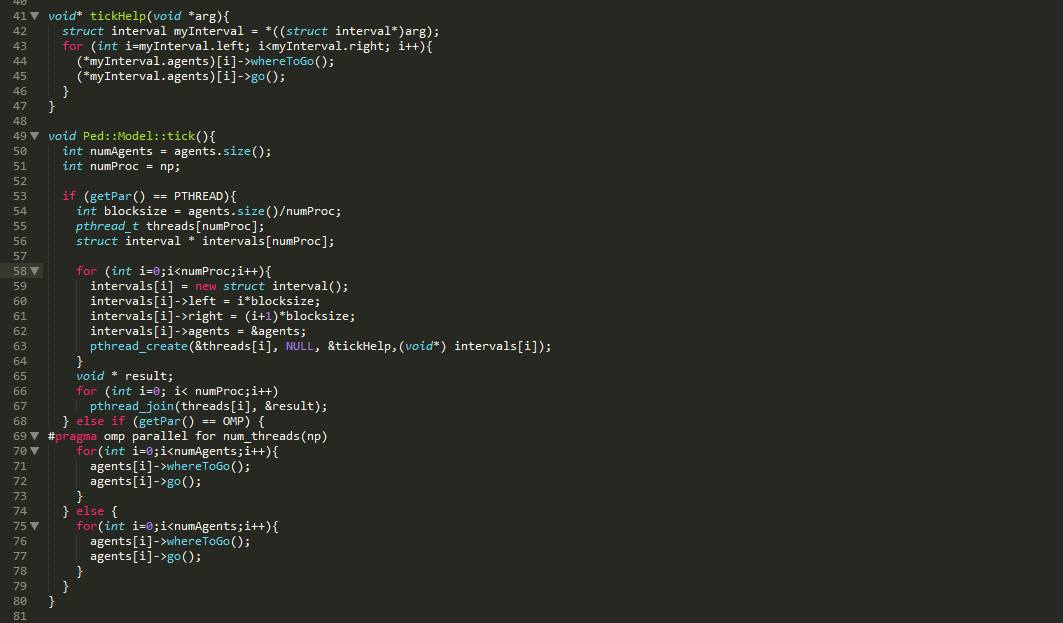
\includegraphics[width=\textwidth]{code.jpg}
	\end{figure}
\end{frame}

\begin{frame}
	\begin{figure}[h!]
	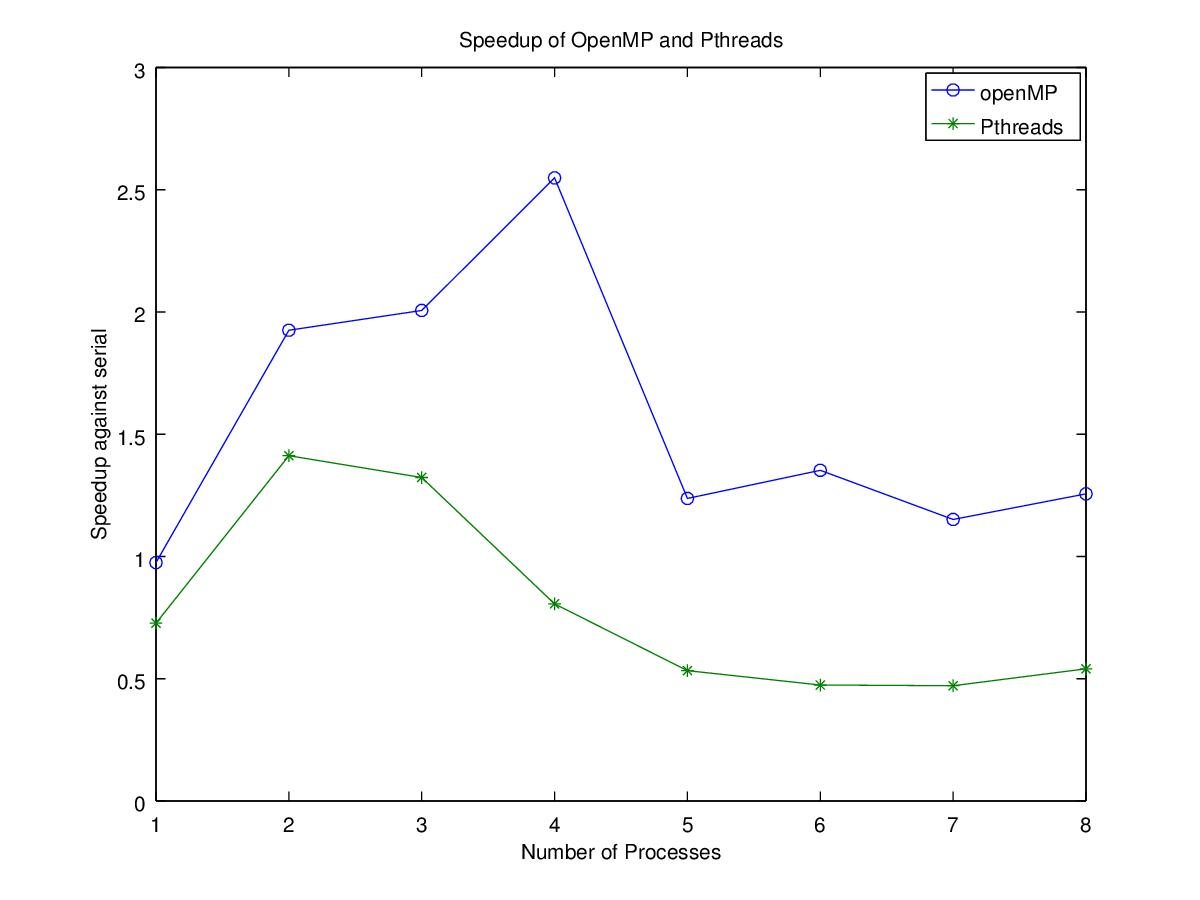
\includegraphics[width=\textwidth]{lab1graph.jpg}
	\caption{Graph showing the speedup of openMP and pthreads for 1 to 8 threads.}
	\end{figure}
\end{frame}


\section{Assignment 2}
\begin{frame}
	\frametitle{Assignment 2}
	\begin{itemize}
	\item
	New data structure: e.g. x[NumOfAgents] instead of agent[i].x
	\item
	New versions of whereToGo() and go(), for vectorization and CUDA
	\end{itemize}
\end{frame}

\begin{frame}
	\begin{figure}[h!]
	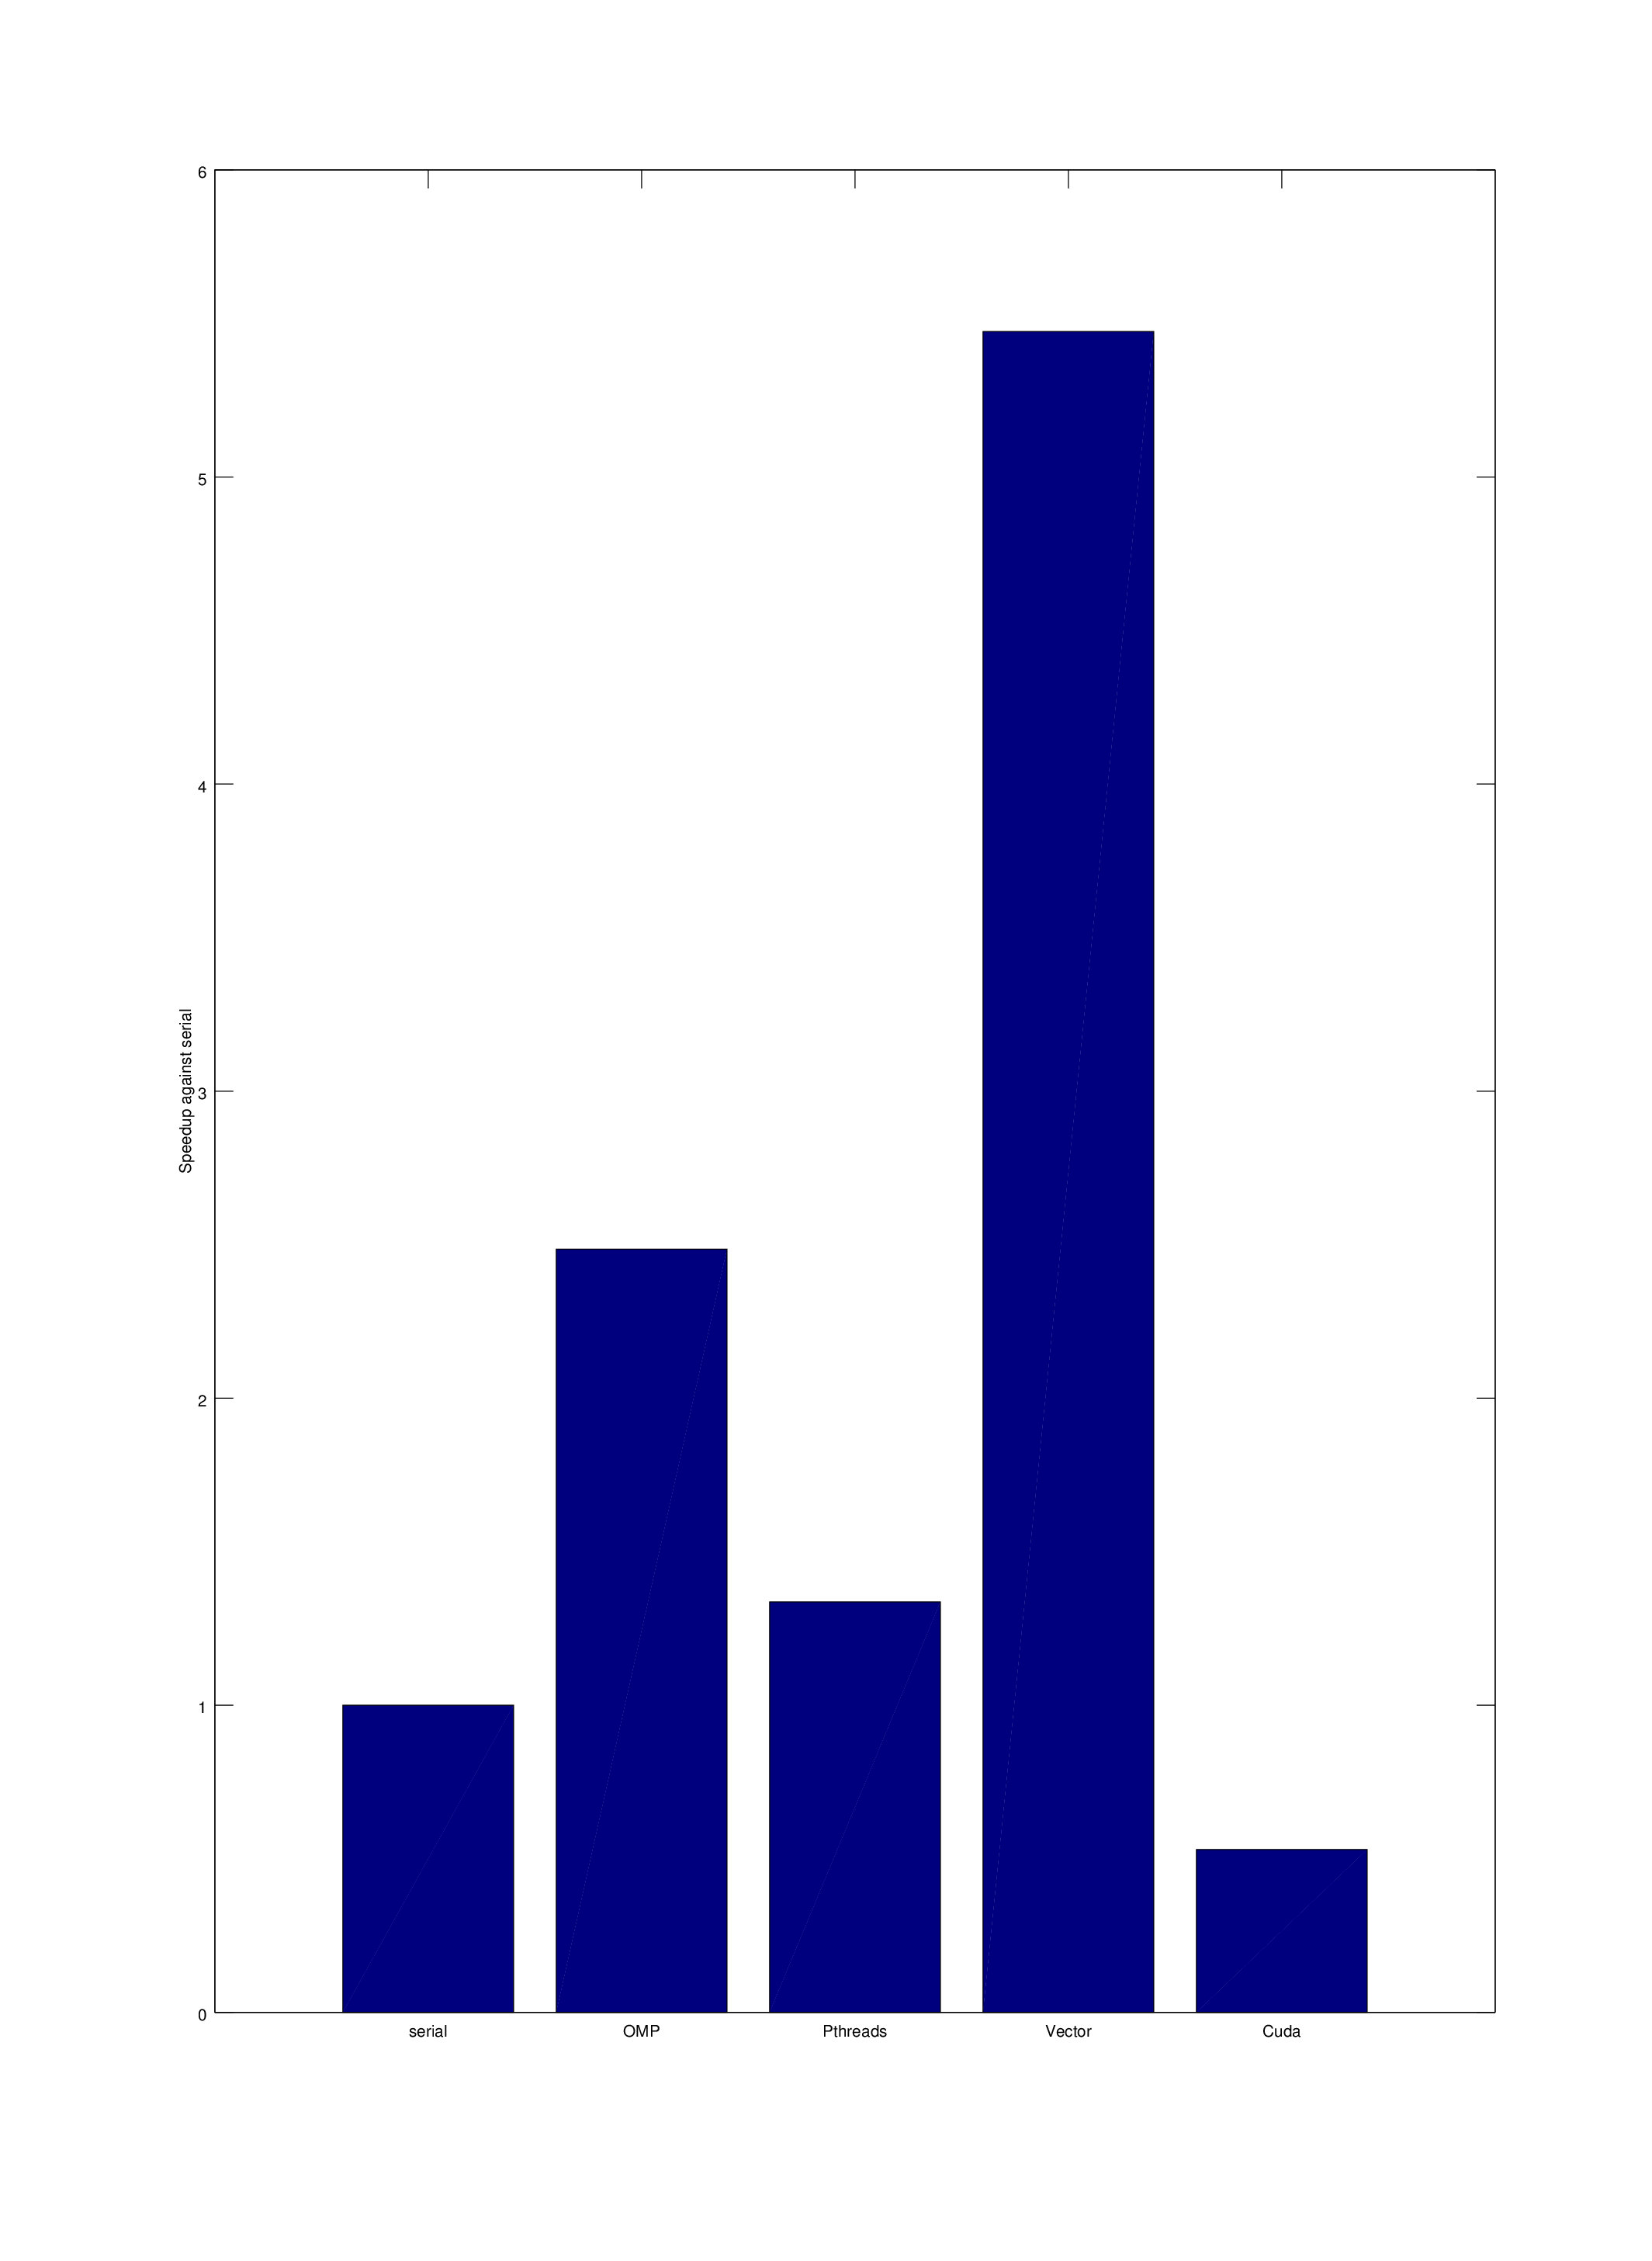
\includegraphics[width=0.5\textwidth]{lab2graph1.png}
	\caption{Speedup 2048 agents}
	\end{figure}
\end{frame}

\begin{frame}
	\begin{figure}[h!]
	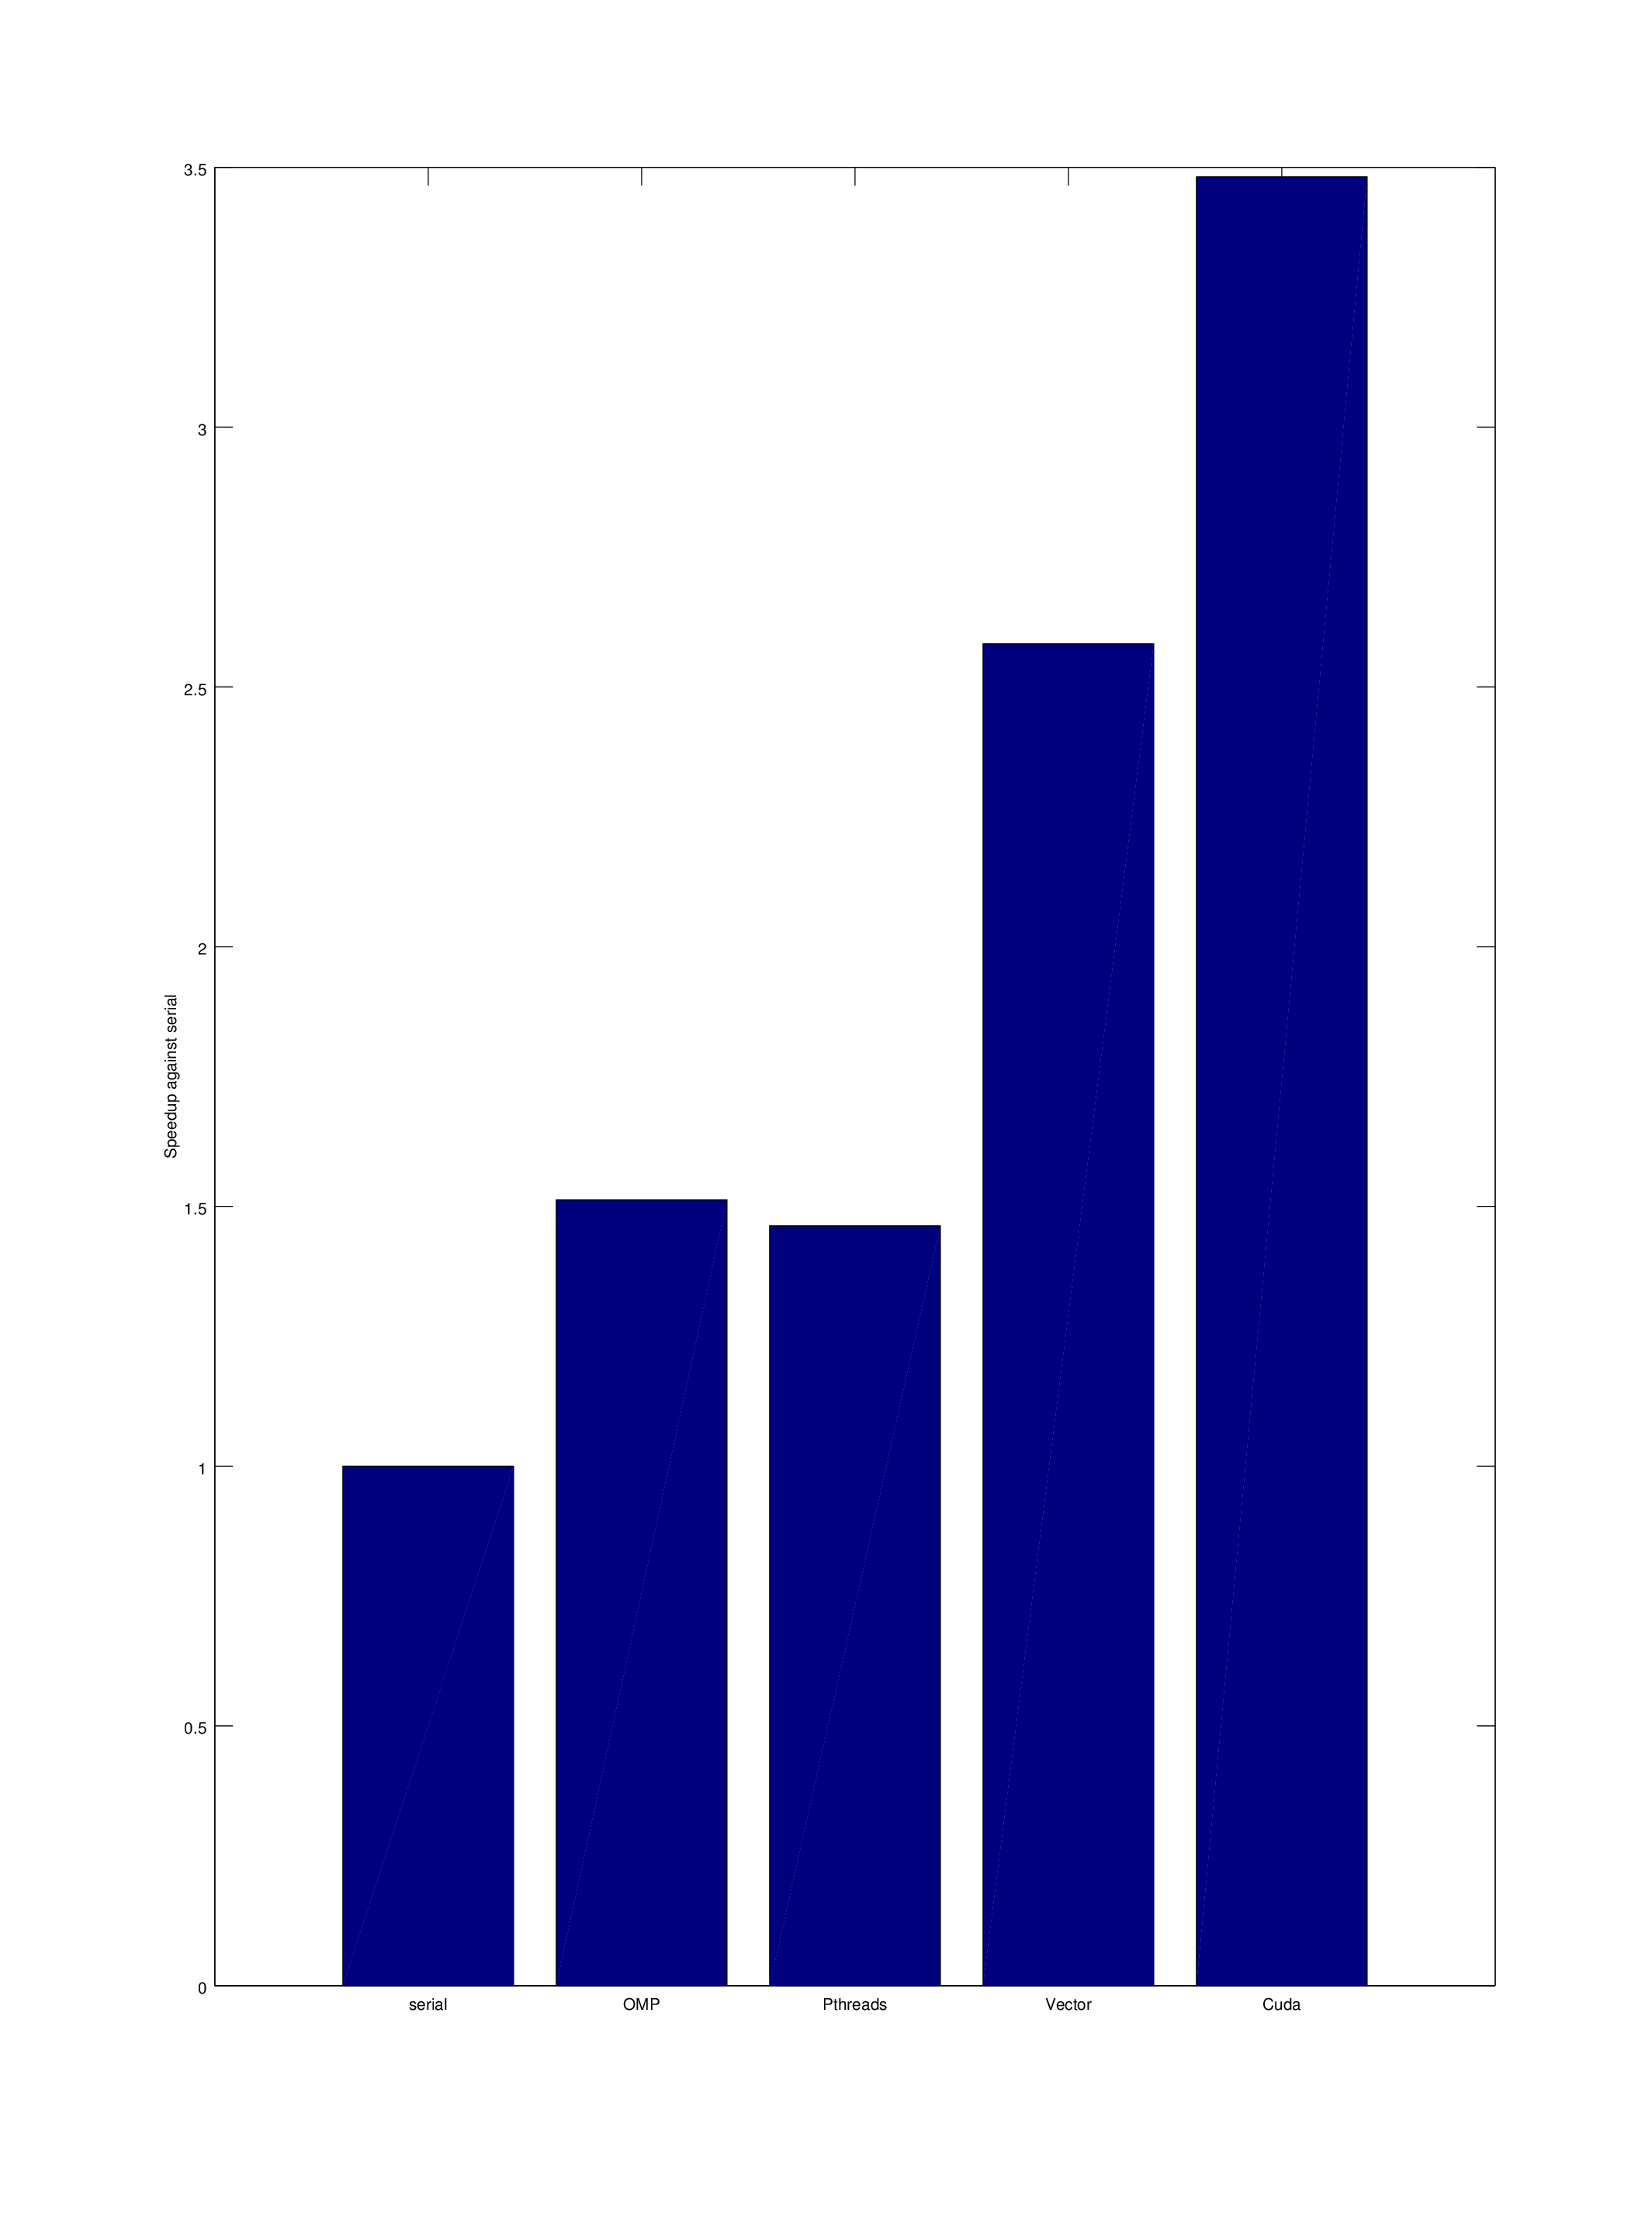
\includegraphics[width=0.5\textwidth]{lab2graph2.png}
	\caption{Speedup 480000 agents}
	\end{figure}
\end{frame}

\section{Assignment 3}
\begin{frame}
	\frametitle{Assignment 3}
	\begin{itemize}
	\item
	Exchanged the tree structure to a simple 2d grid
	\item
	Two solutions: region-based pthreads implementation and simple omp pragma
	\end{itemize}
\end{frame}

\begin{frame}
	\begin{figure}[h!]
	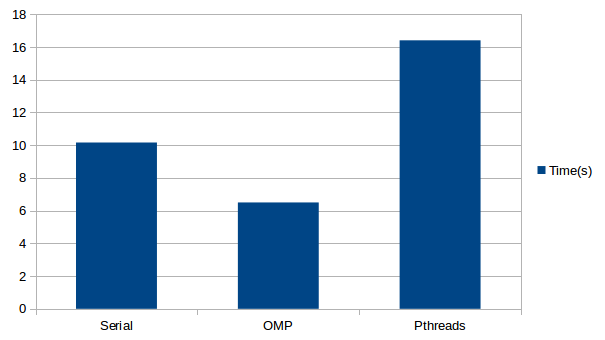
\includegraphics[width=\textwidth]{lab3graph1.png}
	\caption{Runtime 2048 agents (before duplicates)}
	\end{figure}
\end{frame}

\begin{frame}
	\begin{figure}[h!]
	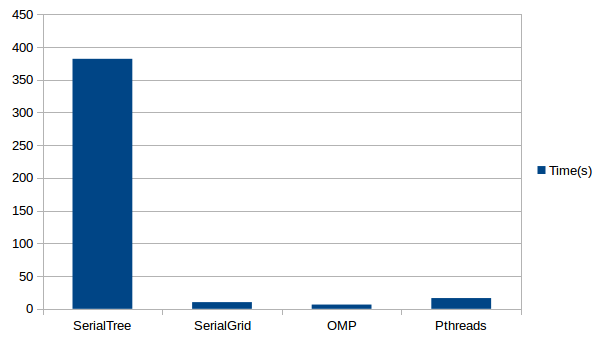
\includegraphics[width=\textwidth]{lab3graph2.png}
	\caption{Runtime 2048 agents (before duplicates)}
	\end{figure}
\end{frame}

\section{Assignment 4}
\begin{frame}
	\frametitle{Assignment 4}
	Four CUDA kernels:
	\begin{itemize}
	\item
	Fading the heatmap 
	\item
	Updating the heatmap with agent information
	\item
	Scaling the heatmap
	\item
	Adding a gaussian blur filter to the heatmap
	\end{itemize}
\end{frame}

\begin{frame}
	\begin{figure}[h!]
	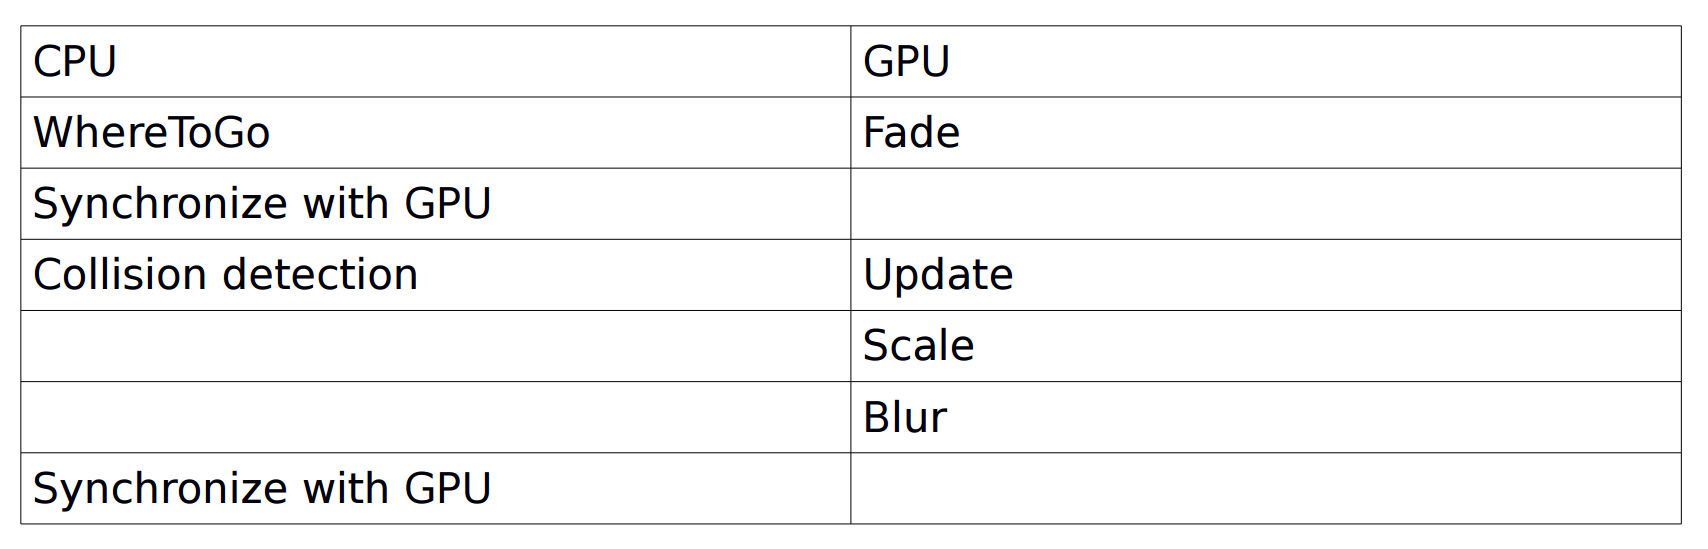
\includegraphics[width=\textwidth]{lab4graph1.png}
	\end{figure}
\end{frame}

\begin{frame}
	\begin{figure}[h!]
	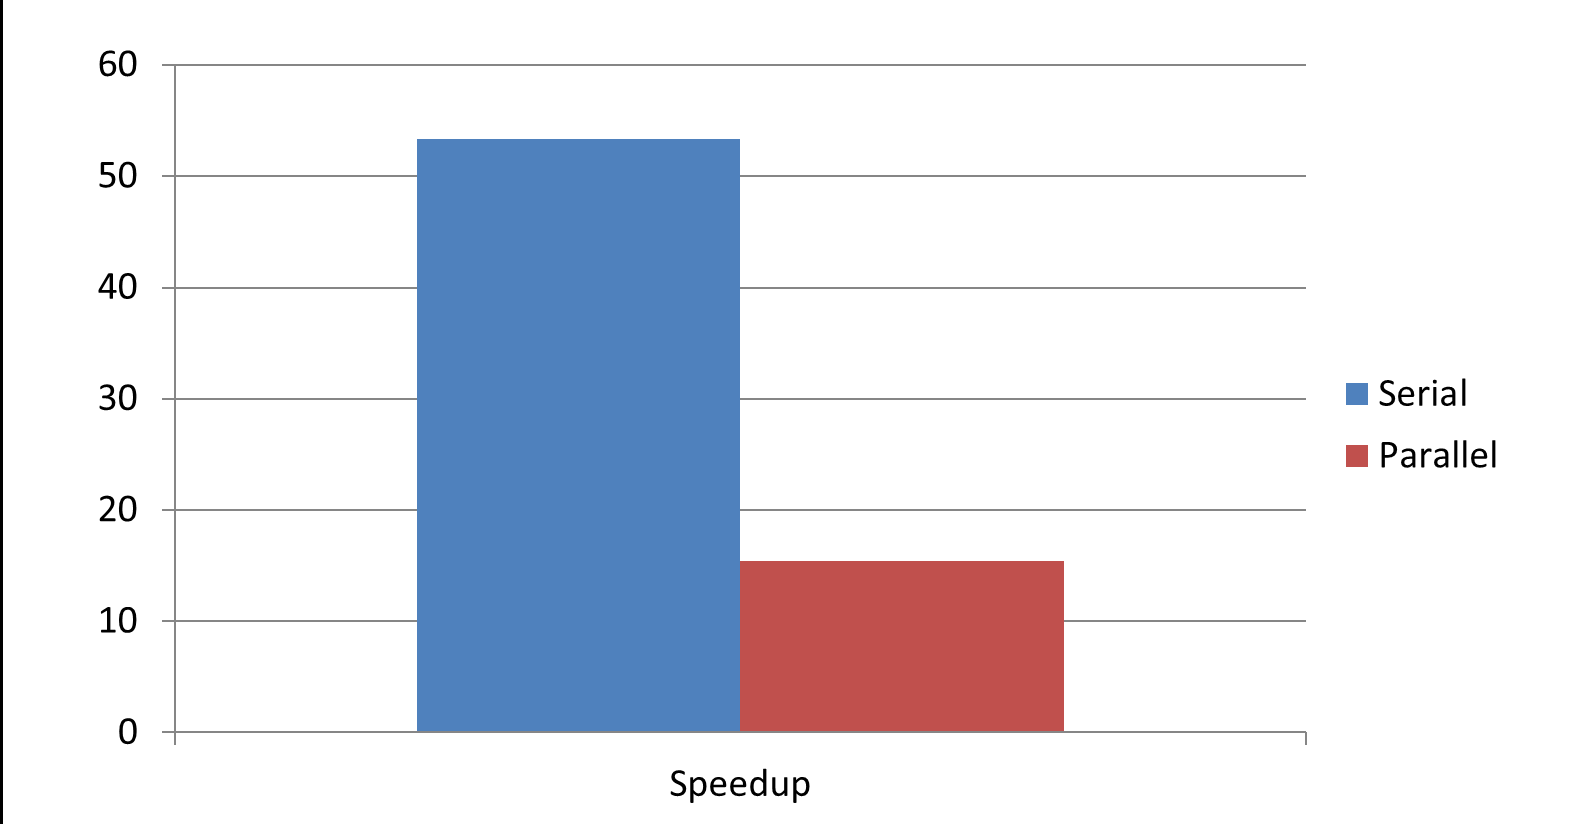
\includegraphics[width=\textwidth]{lab4graph2.png}
	\end{figure}
\end{frame}
\begin{frame}
	\frametitle{Observations}
	\begin{itemize}
	\item
	Cuda could lead to a performance degredation when dealing with small amounts of data, memory allocation overhead, synchronization, etc.
	\item
	Easier to implement and debug with SIMD
	\item
	Parallel execution in CPU and GPU with CUDA
	\item
	Right design can reduce synchronization between CPU and GPU
	\end{itemize}
\end{frame}

\begin{frame}[plain]
	\begin{centering}
	\pgfimage[height=\textheight]{uppsala_logo}
	\par
	\end{centering}
\end{frame}


\end{document}
